Section \ref{section:related_work} has explored the K-Means clustering algorithm, its initialization techniques, approximations to enhance performance, and parallelization methods. We have examined the advantages and disadvantages of each approach and how they can be applied in various contexts. In particular, we have seen that K-Means++ initialization produces better results, but requires an initial time cost, methods operating on samples of the entire dataset improve performance but decrease the quality of the results, and parallelization improves performance but does not always scale as expected due to diminishing returns. Our goal is to solve these trade-offs, and to have a method able to increase performance without sacrificing the quality of the results, and without paying an initial time-cost.  In order to accomplish this, we suggest breaking the cyclic dependency existing in K-Means, highlighted in section 2, by using Speculation. 

\subsection{Breaking K-Means dependencies}
\label{section:breaking_dependencies}
We saw how Algorithm \ref{alg:1} consists of two main steps: the assignment step and the update step. The assignment step includes \ref{alg:step:3} and \ref{alg:step:4}, while the update step includes \ref{alg:step:5}. The two steps are dependent on each other, as the assignment of data points depends on the current cluster centers, which are in turn updated based on the assignments. This creates a cyclical pattern in the K-Means algorithm.

We can group the K-Means steps into stages, each containing an Assignment step and
an Update step. Many of these stages are repeated in the K-Means algorithm until convergence.
A first way of breaking the highlighted dependencies would be to separate in each stage the Update and Assignment into two different processes. This corresponds to the approach used in \cite{Sioulas:282304}, and it aims to run in parallel the Assignment and the Update step, thus reducing the overall time of execution of a single stage. In particular, we would speculate the result of the Assignment (or the Update) allowing the consequent Update (or the Assignment) to start running concurrently. Finally, we could perform a repair stage once the correct result of the Assignment (or the Update) is available. Repeating this procedure for each stage until convergence would result in an overall faster K-Means algorithm.

However, after a study of the time of executions, we can see how the Assignment step takes more time than the Update step. In particular, the ratio between the time of an Assignment step and the time of the Update step increases with $k$, as shown in Figure \ref{fig:ratio_k}. As consequence, the parallelization of Assignment and Update in each stage results inefficient, since the gain of the concurrent execution is irrelevant for $t_{Assignment} \gg t_{Update}$.

\begin{figure}[ht]
\centering
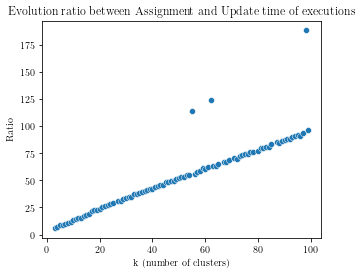
\includegraphics[width=\linewidth]{./plots/ratio_k.png}
\caption{Evolution of ratio between time execution of Assignment and Update}
\label{fig:ratio_k}
\end{figure}

Therefore, we decided to use a different approach in the implementation of Speculation. Instead of running Assignment and Update in parallel for each stage, we run two executions of K-Means concurrently. Both executions start with the same given centroids, but there are two distinct executions: the slow execution, which processes one stage consisting of one Assignment stage and one Update step using the full dataset, and the fast execution, which runs on a sample of the dataset and is able to process multiple stages in the same amount of time as the slow execution. As soon as the slow execution finishes, the fast execution is interrupted, to guarantee that they both take the same amount of time.
Finally, we compare the centroids proposed by both the executions, we compute the inertia they lead to on the entire dataset, and we pick the centroids with the smallest inertia.
\begin{algorithm}
\caption{K-Means Clustering using Speculation}
\label{alg:kmeans_speculation}
\begin{algorithmic}[1]
\State Initialize centroids $c_i$ randomly
\State Create two threads of execution: slow and fast
\label{state:create_threads}
\State Run 1 Assignment stage and 1 Update stage on the slow execution starting from $c_i$
\State Run as many as possible stages on a sample of the dataset on the fast execution starting from $c_i$
\State When slow execution finishes, stop fast execution. Get the proposed centroids $c_{slow}$, $c_{fast}$
\State Compute the inertia $I_X(c_{slow})$, $I_X(c_{fast})$ on the entire dataset $X$
\State $c_i = argmin_c(I_X(c_{slow}), I_X(c_{fast}))$ select centroids minimizing the inertia.
\label{state:select_centroids}
\While{not (centroids no longer move | a maximum number of iterations is reached)}
    \State repeat \ref{state:create_threads} to \ref{state:select_centroids}
\EndWhile
\State Return the final clusters and centroids
\end{algorithmic}
\end{algorithm}

The fast execution of the K-Means algorithm is used to speculate and predict an approximation of future centroids that the slow execution may encounter, by traversing a speculative path. In case its prediction is correct, it will allow skipping several stages of the K-Means algorithm, breaking this way the cyclic dependency. This is possible since it works on a subset of the dataset, allowing it to execute faster and dive deeper into the algorithm, approaching more the convergence. However, as shown in section \ref{section:approximation}, this approach can lead to less accurate results when applied to the full dataset due to the use of subsets of the data.
To address this issue, the slower execution is employed to compute the result using the entire dataset, ensuring that Speculative K-Means will converge towards a solution that takes into account the entire dataset. Thus, the two executions have different purposes, with the fast execution being used to speculate and the slow execution being used to ensure accuracy.

In Figure \ref{fig:speculation_conceptual_design},we illustrate the proposed design. We indicate the Assignment stage with $A$ and the Update stage with $B$. The green shapes represent the stages actually executed, whereas the red ones indicate the stages we would save in case the speculation of the fast execution is correct. 

\begin{figure}[ht]
\centering
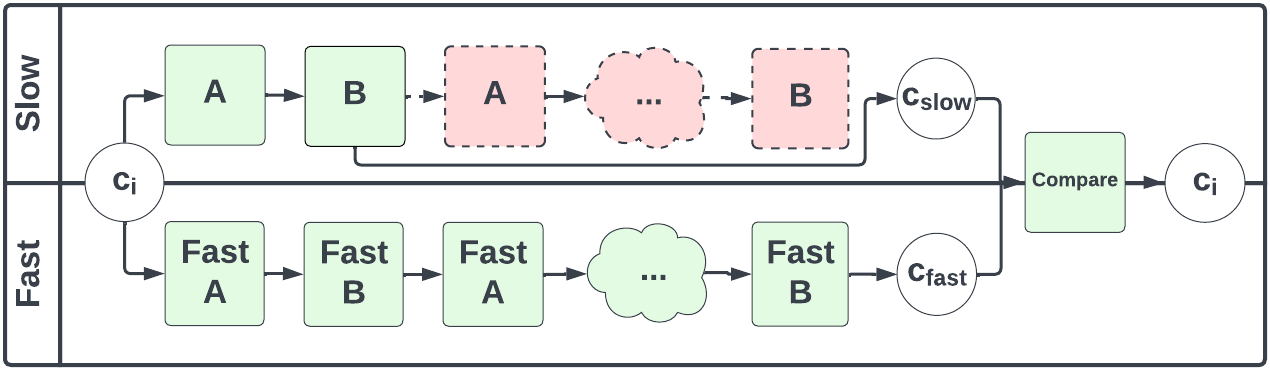
\includegraphics[width=\linewidth]{./plots/speculative_KMeans_conceptual_design.png}
\caption{Conceptual Design of Speculative K-Means}
\label{fig:speculation_conceptual_design}
\end{figure}


The main difference between the Speculative Execution used in \cite{Sioulas:282304}, discussed in section \ref{section:speculation}, and the Speculative K-Means technique is that in the former, the speculation is used to break the dependency between the inner and outer query in order to increase parallelism, while in the latter, the speculation is used to predict possible future results (i.e: the centroids). Therefore, we are breaking the dependencies in a different sense, which is that we are not traversing the entire chain of dependencies anymore in order to arrive at the final result. Additionally, the correction phase in \cite{Sioulas:282304} ensures that the results of the query using the speculation technique are the same as the results of a vanilla execution, while in our approach the correction phase ensure an accurate convergence. The centroids we obtain using the fast execution are an approximation of future centroids with similar inertia we may encounter in the slow execution many stages later, but they are very likely to be different.

\begin{figure}[ht]
\centering
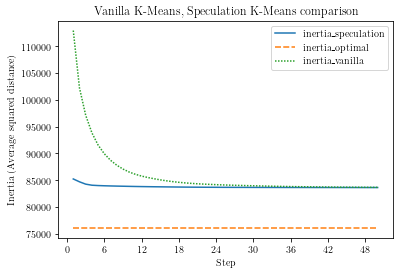
\includegraphics[width=\linewidth]{./plots/vanilla_speculation_comparison.png}
\caption{\href{https://www.openml.org/d/23395}{OpenML Dataset 23395} The dataset used is an ARFF dataset called COMET\_MC\_SAMPLE, version 2, uploaded on April 22nd, 2016. It is publicly available and can be downloaded from the URL provided. It contains 6 features and 89640 instances, and can be found on OpenML with the ID 23395.}
\label{fig:vanilla_speculation_comparison}
\end{figure}
In Figure \ref{fig:vanilla_speculation_comparison}, we can observe the comparison between two K-Means executions, one using Speculation and the other not. Both start from the same initial centroid, compute $k=8$ clusters, and run for a maximum of $50$ stages.
The execution with Speculation is more efficient, as it reaches convergence after 6 stages, while the vanilla implementation takes 30 stages. Furthermore, the accuracy of the final result is the same for both executions, showing how the slow execution and the correction phase ensure a comparable final inertia.


\subsection{Escaping local minima}
\label{section:escaping_local_minima}
Figure \ref{fig:vanilla_speculation_comparison} illustrates that both the Speculative K-Means and the vanilla version do not converge to the optimal minimum. As discussed in Section \ref{alg:K-Means_pp_initialization}, the initialization of K-Means plays a crucial role in determining the quality of the final clustering. Initialization techniques like K-Means++ improve the final results, but have an initial time-cost. We propose an alternative approach that avoids this initial cost, while still leading to a global minimum.

Figure \ref{fig:speculation_conceptual_design} and Algorithm \ref{alg:kmeans_speculation} show how the fast execution starts from the same centroids as the slow execution. However, by doing this, both executions are conditioned by the first initialization of the centroids. We suggest that the fast execution starts from a slightly different set of centroids than the slow one. This would allow us to take advantage of the fast execution to explore more of the solution space, searching for global minima.  At the same time, the repair stage, where we compare the found centroids by computing their inertia, will guarantee convergence. This method is similar to having a vanilla K-Means executed many times from different initial centroids, and picking the best-obtained solution, but it is implemented only on the fast execution, and it is distributed over many speculative executions.

Each time we start the speculation phase, we suggest sampling $k$ datapoints from the dataset as new initial centroids $c_i'$, and modifying the starting centroids of the fast execution by combining linearly the given initial centroids and the sampled ones
\begin{equation}
c_i = p \cdot c_i + (1-p) \cdot c_i'
\end{equation} The value $p$ determines how intensely we want to perturb the initial centroids: the closer it is to $0$ the more random the centroids are, and the more we explore the solution space. This parameter expresses the degree of exploration we want from the fast execution. It can be set statically before the K-Means execution to an optimal value which may vary from dataset to dataset, or it can be adapted at run time, by adapting the randomness based on the quality of solutions we are finding stage after stage.
In Figure \ref{fig:vanilla_speculation_comparison_resampling} we can see how using the centroid resampling technique with $p = 0.8$ improves the inertia of the final clusters.
\begin{figure}[ht]
\centering
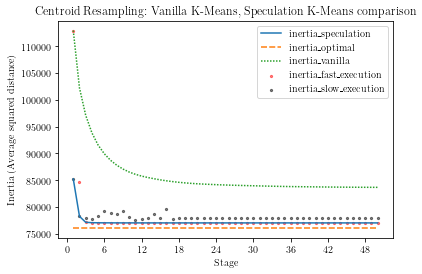
\includegraphics[width=\linewidth]{./plots/vanilla_speculation_comparison_resampling_centroids.png}
\caption{Escaping local minima: Speculative K-Means with centroid resampling. $p = 0.8$}
\label{fig:vanilla_speculation_comparison_resampling}
\end{figure}


\subsection{Speculation in the final stages of K-Means}
\label{section:final_stages}
As the algorithm approaches convergence, the accuracy and effectiveness of the speculation carried out by the fast execution decreases, as shown in Figure \ref{fig:vanilla_speculation_comparison}. In the initial stages, the inertia of the centroids proposed by the fast execution is significantly smaller than the inertia of the centroids of the slow execution, but it becomes comparable in the next 3/4 stages. Additionally, as we approach convergence, the inertia of the fast execution's centroids is constantly greater than that of the slow execution.
This is due to the fact that the last stages of K-Means before convergence need the entire datasets in order to compute the exact position of the centroids, and we are not able to do this by using a sample of it.
This leads us to the question of what to do with the fast execution, and if we can improve its prediction even during the last stages before convergence.
We propose several possible approaches.

First, we propose keeping track of the previous predicted centroids by the fast execution. Every time a fast execution starts we sample a different subset of dataset it will work on.
Each subset will lead to a different centroids prediction, therefore we decide to keep memory of them using a tracing method, which consist in updating the newly discovered $c_{fast}$ centroids with the $c_{fast}^{past}$ past centroids in the following way:
\begin{equation}
c_{fast} = q \cdot c_{fast} + (1-q) \cdot c_{fast}^{past}
\end{equation}
Again, we can see how $q$ plays the role of a hyperparameter which determines how much we should keep track of the past speculated centroids.
This type of tracing leads to an exponential decay of the memory of the past centroids.
The reason why this method should help the prediction of the fast execution in the late stages of K-Means, is because it tries to combine the contribution of different speculation. If the problem resides in the fact that a sample of the dataset is not able to represent the entire dataset in the computation of the centroids, then by combining the contribution of different samples we should mitigate this limitation. In Figure \ref{fig:vanilla_speculation_comparison_trace} we can see how with tracing the prediction of the fast execution are more accurate even in the last stages.

\begin{figure}[h]
\centering
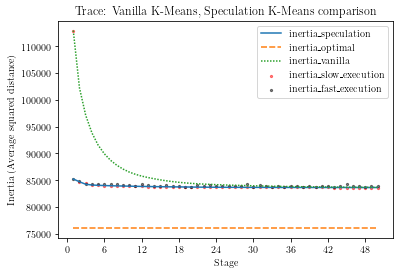
\includegraphics[width=\linewidth]{./plots/vanilla_speculation_comparison_trace.png}
\caption{Speculative K-Means with tracing $q = 0.5$, without centroid resampling.}
\label{fig:vanilla_speculation_comparison_trace}
\end{figure}

An alternative approach that may be effective is to gradually increase the sample size of the data points that the fast execution algorithm is working with. As previously mentioned \ref{section:approximation}, there is a trade-off between performance and accuracy when using subsamples in K-Means, with smaller sample sizes leading to faster stages but less accurate predictions. At the start of the algorithm, it may be beneficial to use a small sample size in order to quickly explore different speculation paths and arrive at centroid estimates that are close to the final solution. In this phase, the accuracy of the predicted centroids is not as important as being able to delve into the speculation path for numerous stages. However, as we approach convergence, it becomes more crucial to have accurate speculation. In this phase, we need to make small adjustments to the centroids in order to find their optimal positions, and in order to do this we need to have access to the full dataset. Thus, we can gradually increase the sample size in order to reduce the number of stages processed by the fast execution (which is not a significant concern at this point, since we are close to convergence) and improve the accuracy of our predictions by having an increasing complete view of the data.

Another solution we propose is to switch to data parallelism in the later stages of the algorithm. If the fast execution is less effective in the final stages, it may be more beneficial to use the resources allocated to it for parallelizing the slow execution, which is the only one capable of finding the final solution. This transition can be done gradually. It's worth noting that, if centroid resampling is used as mentioned in \ref{section:escaping_local_minima}, the fast execution may still be able to find an optimal solution in the final stages. Therefore, it may be important to not switch to full parallelization too early in order to allow the fast execution a chance to find these optimal solutions.
